\section{BDS Model} \label{bds}

\begin{figure*} 
	% \advance\leftskip-1cm 
	\centering
	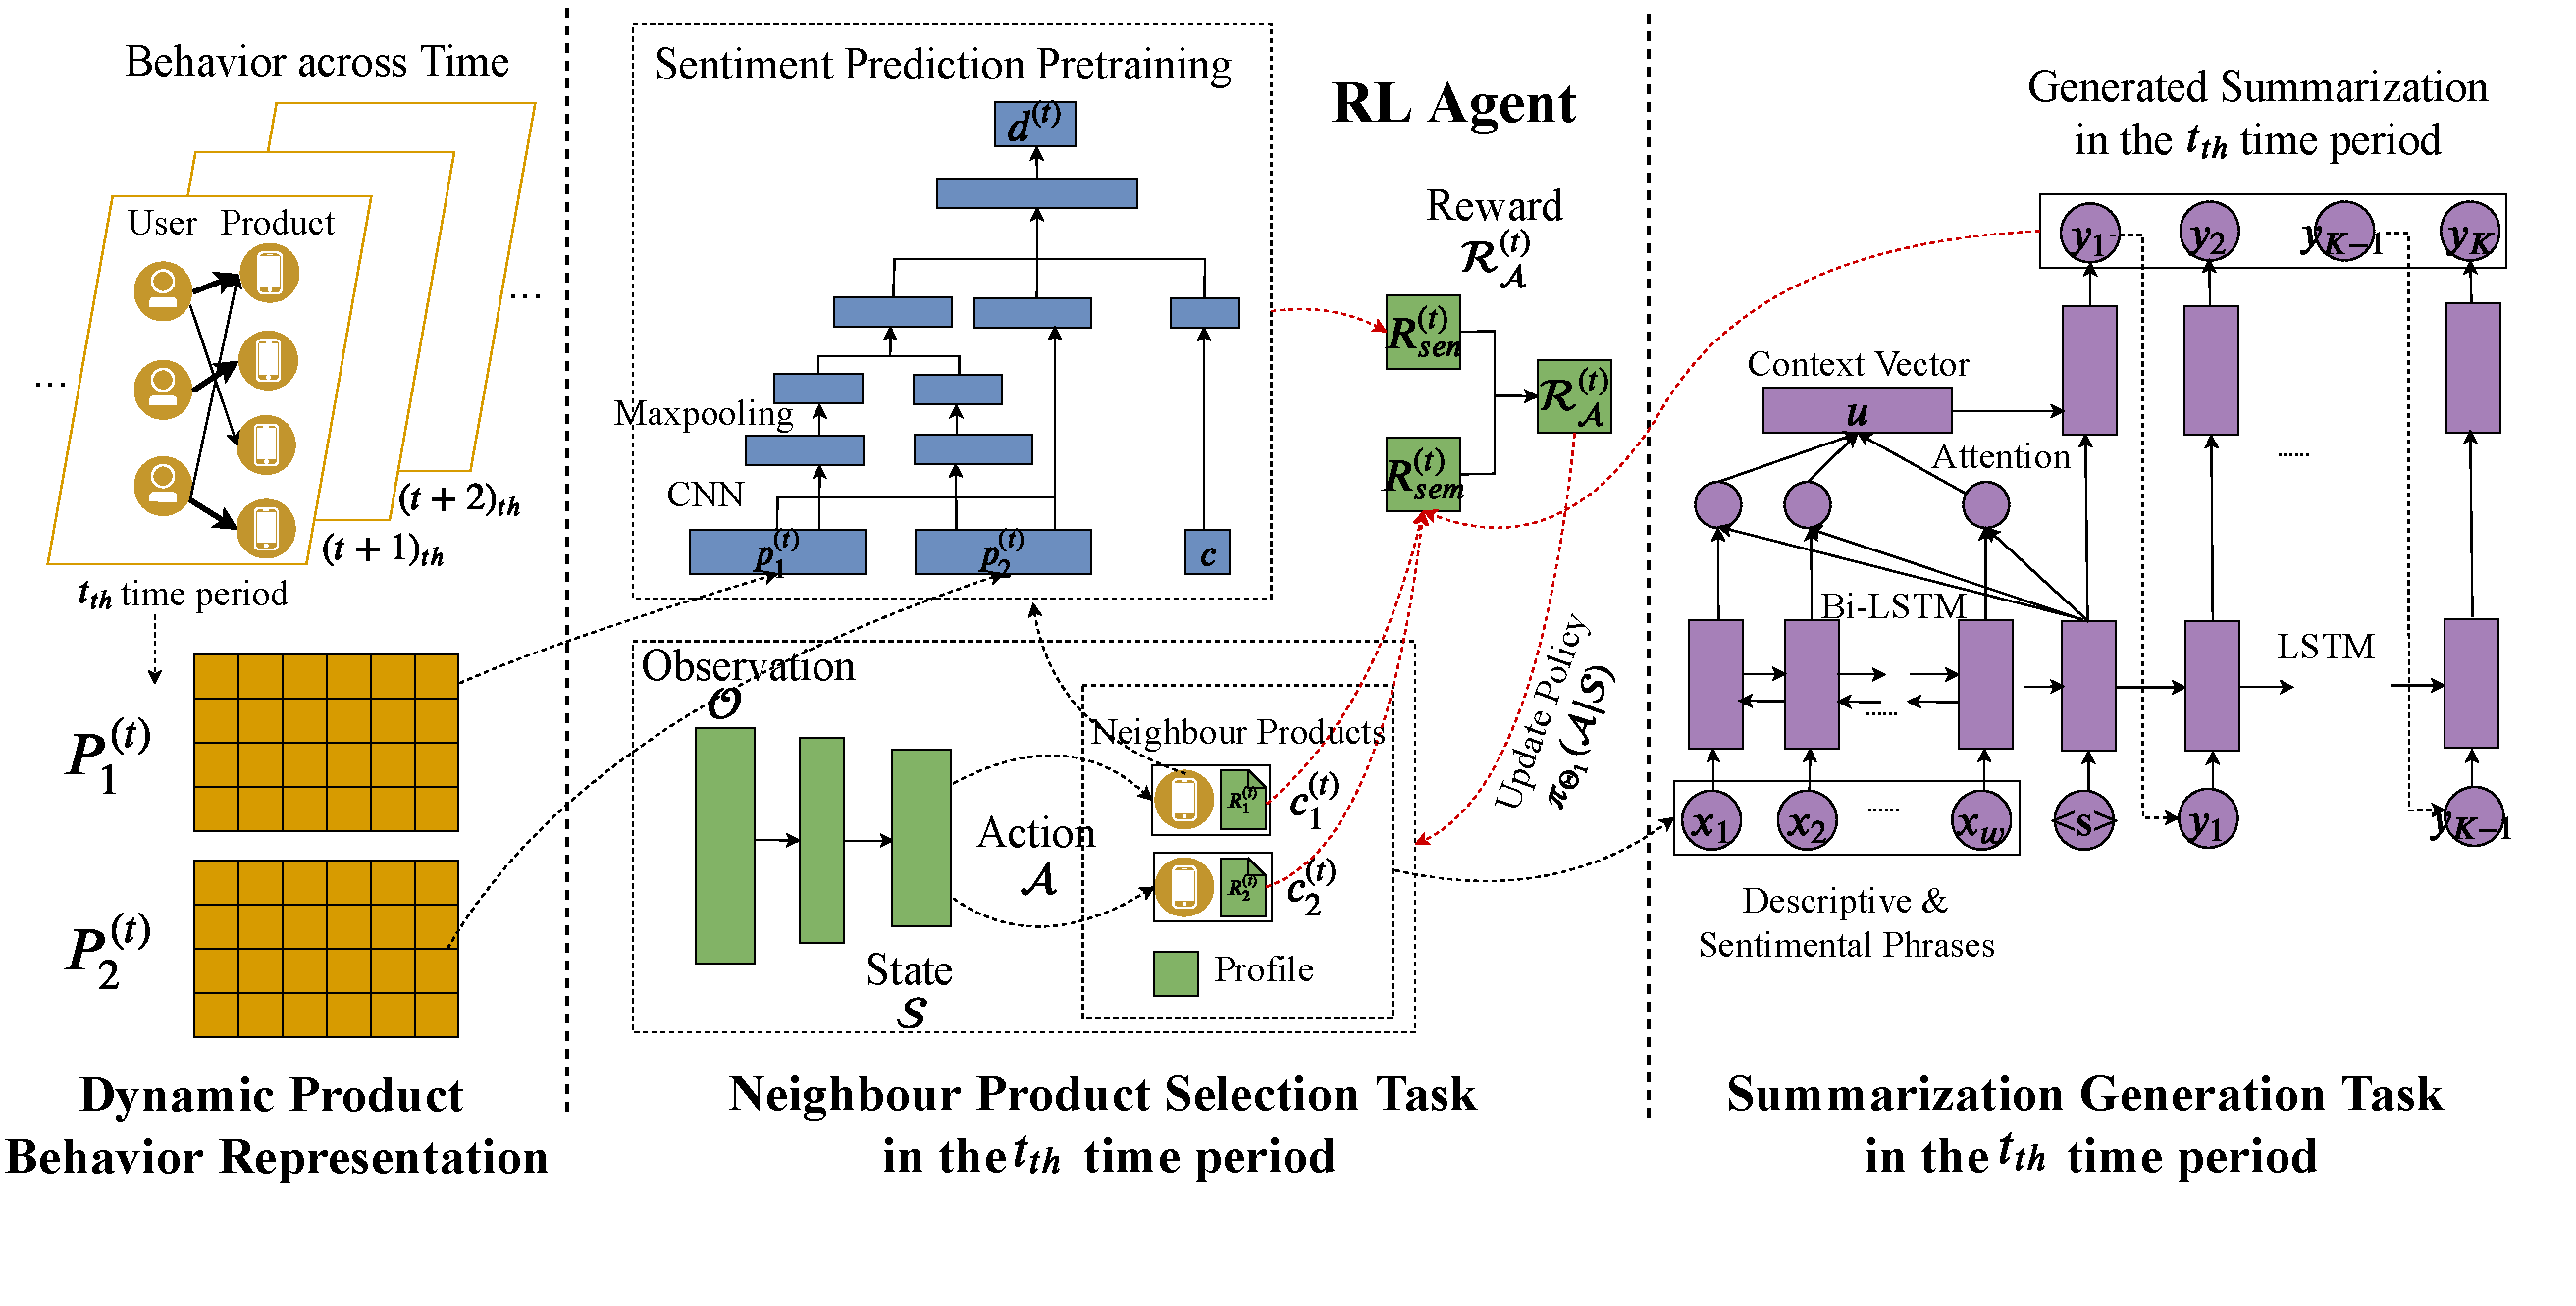
\includegraphics[width=1\textwidth]{img/chapter5/pipeline.pdf}
	\caption{ The overall architecture of BDS model in the $t_{th} $ time period. Each color refers to an individual model component. Dynamic Product Behavior Representation (for all products) and Community Distribution Pretraining (for seed products only) are optimized before training the main multi-task model (Neighbor Product Selection \& Summarization Generation). Red dashed lines show the workflows to calculate RL reward and in return to optimize RL policy. Data Prerequisite steps are omitted here for simplicity but are illustrated in detail in the main paper. }
	\label{fig:c5_pipeline}
\end{figure*}

The overall model architecture is sketched in Figure \ref{fig:c5_pipeline}. My final goal is to generate product dynamic summarizations using behavior data instead of product reviews. To optimize BDS model, the involved data are categorized into two groups: training \& validation data and seed product data. The training \& validation data contains products with both sufficient user behavior and temporal reviews in an individual time period. While seed product data are products required to have sufficient behaviors and reviews across all time periods. The training \& validation data helps to calculate dynamic product behavior presentations (\textit{Section \ref{sc:dpbr}}) and seed product data pretrains community distribution model (\textit{Section \ref{sc:spp}}). Subsequently, a multi-task model dynamically selects neighbor products (\textit{Section \ref{sc:rns}}) from seed products whose sentimental phrases filtered from reviews contribute to generate product summarization (\textit{Section \ref{sc:sgt}}). 

\subsection{Data Prerequisite} \label{sc:dp}

Before optimizing BDS model, four following types of information need to be clarified and extracted as data prerequisite:

\textbf{Seed Products:} The top products having the most sufficient behaviors and reviews across all $t$ time periods are regarded as seed products. Their community distributions are prior-known in each time period, which are later used to guide neighbor product selection (Section \ref{sc:npst}). 

\textbf{Product Descriptive Phrase:} AliNLP\footnote{English Tutorial: https://www.alibabacloud.com/help/product/57736.html \\ Chinese Tutorial: https://data.aliyun.com/product/nlp}, a paid NLP service by Alibaba, can extract name entities and sentimental phrases from E-commerce review contexts. Each product is associated with a description profile. After applying AliNLP Named Entity Recognizer (NER) on their profiles, I only keep the noun phrases to characterize related products.

\textbf{Review Sentimental Phrase:} The AliNLP sentiment analyzer can also extract sentimental phrases related to specific aspects from seed product reviews, i.e., `poor quality' is a sentimental phrases of `\textit{Quality}' aspect. Later on, these filtered sentimental phrases will be concatenated with product descriptive phrases as the model input for product summarization (Section \ref{sc:sgt}).

\textbf{Product Community Distribution:} In this paper, seed product' community distribution is prior knowledge which is learned from their reviews via AliNLP. As user behaviors has strong correlation to product characteristics, their behavior based communities should also be strongly correlated with communities calculated from product reviews which depicts product characteristics. It is a normalized vector in which each dimension represents the product affiliation towards each community, It is the ground truth to guide Community Distribution Pretraining (Section \ref{sc:spp}).  

\subsection{Dynamic Product Behavior Representation} \label{sc:dpbr}

Matrix factorization is utilized on dynamic user behaviors to learn product behavior representation across all time periods. In the initial time period, I learn both user and product $m$ types of behavior representations via related user behavior $\{B^{(0)}_{1},...,B^{(0)}_{m}\}$, where a behavior type can refer to `\textit{Click}' or `\textit{Purchase}', etc. The $i_{th}$ type of user behavior $B^{(0)}_{i}$ is in a format of sparse matrix where each row denotes a user and each column denotes a product. The data points in $B^{(0)}_{i}$ denote users' $i_{th}$ type of behaviors on products. Considering all potential methods listed in \textit{Section \ref{sc:baseline}}, I empirically select Probabilistic Matrix Factorization (PMF) to decompose $B^{(0)}_{i}$ to user representation matrix $U^{(0)}_{i}$ and product representation matrix $P^{(0)}_{i}$ by satisfying the following equation:
\begin{equation}
B^{(0)}_{i} = U^{(0)}_{i} (P^{(0)}_{i})^\intercal, i = 1,...,m
\end{equation}

As user shopping preference is consistently stable, once user representation $U^{(0)}_{i}$ is calculated from the initial period, it remains unchanged and bridges product dynamic behavior representation in subsequent time periods. 

In the $t_{th}$ time period, the matrix form of Least Squares Approximation \cite{nasrabadi2007pattern} helps to calculate the $i_{th}$ type of product behavior representation $P^{(t)}_{i}$ given related user behavior $B^{(t)}_{i}$ and user consistent representation $U^{(0)}_{i}$:
 
\begin{equation}
\begin{aligned} 
& B^{(t)}_{i} = U^{(0)}_{i} (P^{(t)}_{i})^\intercal, i = 1,...,m \\
& \Rightarrow (U^{(0)}_{i})^\intercal (B^{(t)}_{i} - U^{(0)}_{i} (P^{(t)}_{i})^\intercal) = 0 \\
& \Rightarrow (U^{(0)}_{i})^\intercal U^{(0)}_{i} (P^{(t)}_{i})^\intercal = (U^{(0)}_{i})^\intercal B^{(t)}_{i} \\ 
& \Rightarrow (P^{(t)}_{i})^\intercal = (( U^{(0)}_{i})^\intercal U^{(0)}_{i})^{-1}(U^{(0)}_{i})^\intercal B^{(t)}_{i} \\
& \Rightarrow P_{i}^{(t)} = (B_{i}^{(t)})^\intercal U^{(0)}_{i}(( U^{(0)}_{i})^\intercal U^{(0)}_{i})^{-1}
\end{aligned}
\end{equation}


\subsection{Neighbor Product Selection Task}\label{sc:npst}

\subsubsection{Community Distribution Pretraining} \label{sc:spp}

This pretraining process is only leveraged on seed products. In the $t_{th}$ time period, I combine product behavior representation and category to estimate product community distribution via a hybrid CNN-MLP (Convolutional Neural Network and Multilayer Perceptron) approach. Let $c$ be the category of a target product, stored originally as one-hot embedding. To better represent its enriched information, I first apply an one-layer MLP with $\rm tahn(\cdot)$ activation function to convert it as a dense vector $v^{c}$.

\begin{equation}
v^{c} = {\rm tahn}(W^{c}c+b^{c})
\end{equation}

where $W^{c}$ and $b^c$ denote the weight matrix and bias respectively.

For the same product, I can also obtain its multi-type behavior representation $\{p^{(t)}_{1},...,p^{(t)}_{m}\}$, where $p^{(t)}_{m} \in P^{(t)}_{m}$ denotes its $m_{th}$ type behavior representation. As CNN kernel can help to filter out the most important dimensions (local features) from a vector, a CNN layer ${\rm cnn}(\cdot)$ with Max pooling mechanism ${\rm max\_pooling}(\cdot)$ is applied to capture product $i_{th}$ type local feature representation $l^{(t)}_{i}$.
\begin{equation}
% \vspace{-0.5em}
\begin{aligned} 
&l^{(t)}_{i} = {\rm max\_pooling}({\rm tahn}({\rm cnn}(p^{(t)}_{i}))), i= 1,...,m
\end{aligned} 
\end{equation}


Subsequently, I average all $m$ types of local feature representation to a single vector $l^{(t)}$. Similarly, I calculate the average product behavior vector $p^{(t)}$ as global feature representation of $m$ types of behaviors: 
\begin{equation}
\begin{aligned} 
&l^{(t)} = \frac{1}{m}\sum_{i = 1}^{m}l^{(t)}_{i} \\
&p^{(t)} = \frac{1}{m}\sum_{i = 1}^{m}p^{(t)}_{i} 
\end{aligned} 
\end{equation}

In the end, a product has three types of information representation, including global feature representation $p^{(t)}$, local feature representation $l^{(t)}$, and category representation $v^{c}$. I concatenate all these information to calculate the estimated product community distribution $d^{(t)}$ over all pre-selected aspects via one layer MLP normalized by $\rm softmax(\cdot)$ function:
\begin{equation}
d^{(t)} = {\rm softmax}(W^{d}[p^{(t)},l^{(t)},v^{c}]+b^{d})
\end{equation}
where $W^{d}$ and $b^{d}$ are related weight matrix and bias. $[\,, ]$ denotes the concatenation operation. 

This pretraining process is optimized by minimizing the cross entropy between the estimated product community distribution $d^{(t)}$ and the actual product community distribution calculated from product reviews (Section \ref{sc:dp}). This optimization step has to be done ahead of the main multi-task model introduced in the following sections. In the later training process, for all products in the training \& validation dataset, their estimated community distribution can be calculated from the optimized pretraining model.

\subsubsection{Reinforcement Neighbor Selection} \label{sc:rns}

In the $t_{th}$ time period, among $h$ seed products with sufficient reviews, a policy gradient approach earns an action to select $s$ neighbor products $\mathcal{A} = \{\alpha_{1}^{(t)},\alpha_{2}^{(t)},...,\alpha_{s}^{(t)}\}$ out of $h$ candidates where $\alpha_{s}^{(t)}$ denotes the $s_{th}$ selected neighbor product. As I do not consider the sampling sequence on neighbor products, the reinforcement approach is a one-step Markov Decision Process (MDP) with single state $\mathcal{S}$ and single action $\mathcal{A}$. 

Assume there are $n$ products in total across all time periods, given a target product, the initial observation $\mathcal{O}$ is the product itself, represented as a one-hot embedding $\in \mathbb{R}^{n}$. The state $\mathcal{S}$ is learned via a two-layer Multilayer Perception (MLP) on the initial observation $\mathcal{O}$:
\begin{equation}
\label{eq:state}
\mathcal{S} = {\rm softmax} (W_{2}{\rm tahn}(W_{1}\mathcal{O} + b_{1}))
\end{equation} 
where $W_1$,$W_2$ and $b_1$ denote related weight matrices and bias, respectively. 

The learned state $\mathcal{S} \in \mathbb{R}^{h}$ is the selection probability distribution over $h$ seed products. Assuming an action is taken to sample $s$ neighbor products with related probability weights $\{\omega_{1}^{(t)},\omega_{2}^{(t)},...,\omega_{s}^{(t)}\} \in \mathcal{S}$, the sampling policy $\pi_{\Theta_{1}}(\mathcal{A}|\mathcal{S})$ can be therefore calculated as:
\begin{equation}
\pi_{\Theta_{1}}(\mathcal{A}|\mathcal{S}) = s!\prod_{i=1}^{s}\omega^{(t)}_{i}
\end{equation} 
$\Theta_{1}$ denote the parameters to be learned. The factorial of $s$ ($s!$) denotes the number of permutations for the selected neighbor products as the neighbor products are sequence insensitive. $\prod_{i=1}^{s}\omega^{(t)}_{i}$ is the generative probability of each permutation. 

To assess the fitness of the $s$ selected neighbor products for the target product, I design two dynamic rewards: a community reward to measure the community similarity, and a semantic reward to calculate the content similarity between $s$ neighbor products and the target product.

\textbf{Community Reward:} 
In the $t_{th}$ time period, I estimate the target product's community distribution as $d^{(t)}_{a}$ by the Community Distribution Pretraining (Section \ref{sc:spp}). The community distributions of all its selected neighbor products $\{d^{(t)}_{1},...,d^{(t)}_{s}\}$ are known as prior knowledge (Section \ref{sc:dp}). To evaluate pairwise distribution similarity, Pearson correlation calculates the community reward $ \mathcal{R}_{com,i}^{(t)}$ of the $i_{th}$ selected neighbor product $\alpha_{i}^{(t)}$ as follows:

\begin{equation}
\mathcal{R}_{com,i}^{(t)} = \frac{\mathbb{E}[(d_{a}^{(t)}-\mu(d_{a}^{(t)}))(d_{i}^{(t)}-\mu(d_{i}^{(t)}))]}{\sigma(d_{a}^{(t)})\sigma(d_{i}^{(t)})}, i = 1,...,s
\end{equation}

where $\mathbb{E}(\cdot)$ denotes the expectation, $\mu(\cdot)$ denotes the mean and $\sigma(\cdot)$ denotes the standard deviation. Larger similarity score offers a higher reward to the related neighbor product.

\textbf{Semantic Reward:} In the $t_{th}$ time period, the semantic reward of neighbor products is measured by the accuracy of generated product summarization. In this paper, we use the word level Jaccard Similarity as the indicator to calculate the semantic reward $\mathcal{R}_{sem}^{(t)}$ for all selected neighbor products, which contains two parts: the averaged Jaccard Similarity between all neighbor product original reviews and real product summarization, and the Jaccard Similarity between generated product summarization and actual product summarization:

\begin{equation}
\mathcal{R}_{sem}^{(t)} = \frac{1}{s}\sum_{i=1}^{s} \frac{|R_{i}^{(t)} \cap Y^{(t)}|}{|R_{i}^{(t)} \cup Y^{(t)}|} + \frac{|\hat{Y}^{(t)} \cap Y^{(t)}|}{|\hat{Y}^{(t)} \cup Y^{(t)}|} 
\end{equation}

where $R_{i}^{(t)}$ denotes all original reviews of the $i_{th}$ neighbor product $\alpha_{i}^{(t)}$, $\hat{Y}^{(t)}$ denotes the generated summarization of target product, and $Y^{(t)}$ denotes its actual summarization. The total reward $\mathcal{R}^{(t)}_{\mathcal{A}}$ of neighbor products is the weighted sum between community reward and semantic reward controlled by a weighting factor $\gamma$:


\begin{equation}
\mathcal{R}^{(t)}_{\mathcal{A}} = \sum_{i=1}^{s} \omega_{i}^{(t)}\mathcal{R}_{com,i}^{(t)} +\gamma \mathcal{R}_{sem}^{(t)}
\end{equation}

\textbf{Task Optimization:} I use policy gradient method to optimize the sampling policy, aiming to maximize the expected total reward for neighbor products. The expected reward $\mathcal{J}_{sel}(\Theta_{1})$ in the $t_{th}$ time period is:

\begin{equation}
\begin{aligned}
\mathcal{J}_{sel}(\Theta_{1}) &= \mathbb{E}_{\mathcal{A} \sim \pi_{\Theta_{1}}(\mathcal{A}|\mathcal{S})}[\mathcal{R}^{(t)}_{\mathcal{A}}]
\end{aligned}
\end{equation}

Then, the gradient is estimated using the likelihood ratio trick:

\begin{equation}
\label{eq:loss_1}
\begin{aligned}
\nabla_{\Theta_{1}}\mathcal{J}_{sel}(\Theta_{1}) &= \nabla_{\Theta_{1}} \sum_{\mathcal{A}} \pi_{\Theta_{1}}(\mathcal{A}|\mathcal{S}) \mathcal{R}^{(t)}_{\mathcal{A}}\\
&\approx \frac{1}{N} \sum_{i=1}^{N}\nabla_{\Theta_{1}}log\pi_{\Theta_{1}}(\mathcal{A}_{i}|\mathcal{S})\mathcal{R}^{(t)}_{\mathcal{A}_{i}}
\end{aligned}
\end{equation}

where $\mathcal{A}_{i}$ denotes the $i_{th}$ of $N$ randomly sampled actions (selecting $s$ neighbor products from $h$ seed products). 

\subsection{Summarization Generation Task} \label{sc:sgt}

In the $t_{th}$ time period, the filtered neighbor product sentimental phrases together with product own descriptive phrases are concatenated into a sequence $X^{(t)} = \{x_{1},...,x_{w}\}$. It is used as the input of Neural Machine Translation (NMT) model to generate product summarization sequence $Y^{(t)} = \{y_{1},...,y_{k}\}$. $w$ and $k$ denote the input and output sequence length, respectively. Filtering out most of emotional and other irrelevant words in advance can better map the input to aspect oriented summarizations instead of subjective review summaries. 

The input sequence $X^{(t)} = \{x_{1},...,x_{w}\}$ is fed one-by-one into the encoder (a single-layer bidirectional LSTM), producing a sequence of encoder hidden states $\{e_{1},...,e_{w}\}$. In decoding step $i$, the decoder (a single-layer unidirectional LSTM) has a decoder hidden state $h_{i}$. Its context vector $u_{i}$ is generated via an Attention mechanism on all encoder hidden states and current decoder hidden state:

\begin{equation}
\begin{aligned}
& a_{ij} = {\rm attention}(h_{i},e_{j}), j = 1,...,w \\
& a_{ij}^{*} = \frac{{\rm exp}(a_{ij})}{\sum_{k=1}^{w} {\rm exp}(a_{ik})}\\
& u_{i} = \sum_{j=1}^{w}a_{ij}^{*}e_{j}
\end{aligned}
\end{equation}
where $a_{ij}$ denotes the attention weight of encoder hidden state $e_{j}$. $a_{ij}^{*}$ is the normalized weight by Softmax function. The weighted sum of all encoder hidden states, $u_{i}$, is the context vector for current step $i$, reflecting the auxiliary information from input sequences.

A one-layer MLP is subsequently utilized on the combination of context vector $u_{i}$ and decoder hidden state $h_{i}$ to generate the vocabulary probability distribution $P_{vocab}$:

\begin{equation}
P_{vocab} = {\rm softmax}(W^{o}[u_{i},h_{i}]+b^{o})
\end{equation}
where $W^{o}$ and $b^{o}$ are related weight and bias.

In decoding step $i$, the generation loss for target word $y_{i}$ is its negative log likelihood, $-logP_{vocab}(y_{i})$. The overall generation loss $\mathcal{J}_{gen}(\Theta_{2})$ is the average of all $k$ step generation losses and $\Theta_{2}$ are all related parameters to be optimized.

\begin{equation}
\mathcal{J}_{gen}(\Theta_{2}) = \frac{1}{k}\sum_{i=1}^{k} -logP_{vocab}(y_{i})
\end{equation}

In the multi-task model, $\mathcal{J}_{sel}(\Theta_{1})$ and $\mathcal{J}_{gen}(\Theta_{2})$ both need to be minimized during the model training process. Each task is learned separately and alternately after taking a certain number of training data batches in their optimization processes.